%% grundlagen.tex
%% $Id: grundlagen.tex 61 2012-05-03 13:58:03Z bless $
%%

\chapter{Grundlagen}
\label{ch:Grundlagen}
%% ==============================
Wie zuvor erwähnt wird unter den in dieser Arbeit verwendeten Reduktionsregeln zwischen einfacheren und komplexeren Regeln unterschieden. Die komplexeren Nemhauser-Trotter und Kronenregel erstellen während der Anwendung weitere Subgraphen für den Problemgraphen, während Grad$_{0}$-, Grad$_{1}$- und Buss-Regel lediglich den Grad einzelner Knoten betrachtet. Darüber hinaus können die Regeln weiter unterschieden werden. All die zu zuvor genannten Regeln entfernen induzierte Teilgraphen aus dem Graphen, an dem sie angewandt werden. Die Folding-Regel \cite{paper:4} (oder Grad$_{2}$-Regeln) zum Beispiel nicht. Hier werden die Nachbarn $u$ und $v$ eines Knoten $x$ des Grades 2 verschmolzen, vorausgesetzt, es gibt keine Kante zwischen diesen Knoten. Es wird ein neuer Knoten $x'$ mit $N(x') = N(u) \cup N(v) \setminus \{x,u,v\}$ eingesetzt un $k$ verringert. Diese Konstruktion muss dann nach dem Durchlaufen des Algorithmus' wieder entpackt werden, da sonst nach der Reduktion kein äquivalenter Problemgraph entsteht. 
Eine schnelle Laufzeit, um zu entscheiden, ob eine Knotenüberdeckung in einem gegebenen Graphen \emph{G}, Parameter \emph{k} und einer Knontenmenge \emph{n} zu finden ist, wird von Chen et al \cite{paper:4} mit $O(kn + 1.271^{k}k^{2})$ vorgeschlagen, welche allerdings unter anderem die Folding-Regel verwendet; die schnellste bekannte Methode, alle Knotenüberdeckungen eines Graphen zu zählen von Mölle et al \cite{paper:5} mit einer Laufzeit von $O(1.3803^{k})$.

%% ==============================
\section{Knotenüberdeckung}
%% ==============================
\label{ch:Grundlagen:sec:Knotenüberdeckung}
%% ==============================
\section{Einfache Reduktionsregeln}
%% ==============================
\label{ch:Grundlagen:sec:Einfache Reduktionsregeln}
Aus einfachen Beobachtungen über den Problemgraphen lassen sich für einen Graphen $G=(V,K)$ und der natürlichen Zahl $k$ einige Reduktionsregelen ableiten.
\begin{enumerate}
\item Knoten, die isoliert stehen und keine Kanten haben, können aus dem Graphen entfernt werden, da sie nicht zu einer minimalen Knotenüberdeckung gehören können (Grad$_{0}$-Regel)
\item Bei Knoten, die genau eine Kante, beziehungsweise genau einen Nachbarknoten haben, wird der  entsprechende Nachbarknoten automatisch in die Lösungsmenge aufgenommen, da einer der beiden Knoten in der Knotenüberdeckung vorkommt und der Nachbarknoten mindestens den Grad 1 hat, also möglicherweise mehr Kanten abdeckt (Grad$_{1}$-Regel)
\item Knoten mit $k+1$ Kanten, werden der Knotenüberdeckung hinzugefügt, da sonst alle Nachbarknoten aufgenommen werden und somit mehr, als $k$ Knoten in der Lösungsmenge wären (Buss-Regel)
\end{enumerate}
Angewandt an eine Probleminstanz bedeutet das Einsetzen einer der Regeln, dass die entsprechenden Knoten und Kanten von einer weiterführenden Betrachtung ausgeschlossen sind. Buss-Regel und Grad$_{1}$-Regel unterscheiden sich von der Grad$_{0}$-Regel dahingehend, dass das Auslösen einer dieser Regeln auch den Parameter $k$ verringert, da ein Knoten in die Überdeckung aufgenommen wird.
 Das Beispiel in Abbildung \ref{fig:vc} kann durch die wiederholte Anwendung der Regeln sogar gelöst werden:
\begin{enumerate}
\item Es stehen 4 Generatoren zur Verfügung, allerdings hat Haus B 5 ausgehende Leitungen $\Rightarrow$ Buss-Regel: B erhält einen Generator und dessen Leitungen haben Strom.
\item Drei disjunkte Mengen von Häusern (\{E, G, F\}, \{D, C\} und \{A, H\}) bleiben übrig, wo jeweils einmal die Grad$_{1}$-Regel angewandt werden kann. Die 3 restlichen Generatoren werden verteilt, wobei sich bei jeder der Häusergruppen mehrere Möglichkeiten bieten.
\item Es steht kein Generator mehr zur Verfügung und aus der Restmenge {E, G, F} bleibt ein Haus ohne stromlose Leitungen zurück $\Rightarrow$ das Haus wird aus der Betrachtung entfernt und das Problem ist gelöst.
\end{enumerate}
Nach der wiederholten Anwendung der Buss-Regel sind alle Knoten mit mehr als \emph{k} Kanten in der Überdeckung und sind von der weiteren Betrachtung ausgeschlossen und quasi aus dem Graphen entfernt. Jeder übrige Knoten kann also maximal \emph{k} Kanten haben. Wenn nun noch mehr als $k^{2}$ Kanten nicht indiziert sind, kann es keine Lösung dieser Probleminstanz geben, da lediglich \emph{k} Knoten in der Lösungsmenge sein dürfen und somit nur maximal $k^{2}$ Kanten  abdecken. Es bleiben höchstens $2 k^{2}$ Knoten (mit mindestens einer Kante), bei denen noch nicht alle Kanten abgedeckt sind übrig\cite{param}, da jede der Kanten an 2 Knoten hat. Wird nun die Grad$_{1}$-Regel angewandt bis sie nicht mehr greift, sind höchstens $k^{2} + k$ Knoten übrig, da jeder dieser Knoten jetzt zwischen 2 und \emph{k} Kanten hat.
Um einen Knoten aus der Knotenmenge $V$ mit mehr als \emph{k} Kanten zu finden, werden im schlimmsten Fall $k \cdot n (n=|V|)$ Schritte benötigt, da jeder Knoten überprüft werden muss. Falls alle Knoten den Grad \emph{k} haben, wird die Buss-Regel nicht ausgelöst. Ansonsten wird der gefundene Knoten mit all seinen Kanten aus dem Graphen entfernt, was wiederum $d \geq k$(wobei $d$ der größte Grad unter den Knoten aus $G$ ist) Schritte benötigt. Die Grad$_{1}$-Regel benötigt im schlimmsten Fall $2 \cdot n$ Schritte um den Graphen einmal zu durchlaufen, da die Betrachtung eines Knoten abgebrochen werden kann, sobald er mehr als eine oder keine Kante hat, da sie dann für diese Regel uninteressant ist. Wird eine Kante gefunden, kann dessen Nachbarknoten und damit alle von diesem ausgehenden Kanten entfernt werden, also im schlimmsten Fall $d$. Wurde die Buss-Regel vor der Grad$_{1}$-Regel angewandt, bedeutet das, dass maximal \emph{k} Schritte gebraucht werden. Um alle Häuser ohne Leitungen zu entfernen, muss lediglich für jedes Haus überprüft werden, ob es Leitungen hat, also \emph{n} Schritte.

%% ==============================
\section{Nemhauser-Trotter Reduktionsregeln}
%% ==============================
\label{ch:Grundlagen:sec:Nemhauser-Trotter Reduktionsregeln}

Der Nemhauser-Trotter-Regel liegt das Nemhauser-Trotter-Theorem zugrunde \cite{trott}:


\textit{Für einen Graphen} $G=(V,E)$ \textit{können zwei disjunkte Mengen}\ $C_{0}\ und\ V_{0}$ \textit{gefunden werden, sodass}
\begin{enumerate}
\item $C_{0}$ \textit{ in einer minimalen Knotenüberdeckung von G enthalten ist,}
\item \textit{der Teilgraph }$G[V_{0}]$ \textit{eine Knotenüberdeckung} \textit{der Größe} $\leq |V_{0}| / 2$ \textit{ hat,}
\item \textit{und} $VC(G) = VC(G[V_{0}])\cup C_{0}$ \textit{ gilt.}
\end{enumerate}
Nach dem Satz von König und unter Verwendung des Algorithmus' von Hopcroft und Karp \cite{paper:6} können diese Mengen mithilfe des Erstellens eines auf dem Problemgraphen basierenden bipartiten Graphen in Polinomialzeit gefunden werden. Der im Zuge dieser Arbeit verwendete Algorithmus ist wie folgt:

\begin{algorithm}[caption={Nemhauser-Totter-Regel.}, label={alg1}]
$G = (V, E), n:= |V|, m:=|E|, d:= maximaler\ Grad\ der\ Knoten\ aus\ G$
Bipartiten Graphen erstellen $B = (V, V', E')$ 
  mit $E':= \{\{x,y'\}, \{x', y\} | \{x,y\} \in E\}$ 
Maximum Matching $M$ von $B$ bestimmen 
$C_{B} \leftarrow VC(B)$ 
$C_{0} \leftarrow \{x \in V\ |\ x \in C_{B}\ und\ x' \in C_{B} \}$ 
$V_{0} \leftarrow \{x \in V\ |\ entweder\ x \in C_{B}\ oder\ x' \in C_{B} \}$ 
\end{algorithm}

Das Erstellen des Bipartiten Graphen in den Zeilen 1-2 benötigt $n \cdot d$, da der Graph kopiert und jede Kante doppelt eingetragen wird. Zeilen 3-4 brauchen mit dem verdoppelten Graphen durch die Verwendung des Algorithmus' von Hopcroft und Karp $\sqrt{2n} \cdot 2m$ Schritte. Um die Zugehörigkeit der einzelnen Knoten in den Zeilen 5-6 zu bestimmen muss der Graph jeweils lediglich einmal durchgegangen werden, also $2n$ Schritte. Insgesamt ergibt das:
\begin{align}
&\ n \cdot d + \sqrt{2n} \cdot 2m + 2n\\
\Rightarrow &\ O(\sqrt{n} \cdot m)
\end{align}
Die Laufzeitabschätzung von  $O(\sqrt{n} \cdot m)$ entsteht, wenn $d$ als Konstante betrachetet wird. Man sieht, dass die Laufzeit des Algorithmus' hauptsächlich vom Finden des Matchings dominiert wird, der Algorithmus eignet sich also für eine Vorverarbeitung des Graphen in Polynomialzeit.
Ein wichtiger Teil des Algorithmus' ist das Finden eines Maxmimum Matchings. Im Allgemeinen ist ein Matching oder eine Paarung für einen Graphen $G=(V,E)$ eine Menge von Kanten $S \subset E$, für die gilt, dass keine zwei Kanten aus $S$ einen gemeinsamen Knoten haben. Ein Maximal Matching $M$ wiederum ist ein Matching, für das gilt, dass $M$ keine weitere Kante aus $E$ hinzugefügt werden kann, ohne die Matchingeigenschaft zu zerstören. Maximum Matchings erfüllen die Eigenschaften eines Maximal Matchings und enthalten außerdem die Größte Anzahl an Kanten, im Vergleich zu anderen Matchings.\\
Mit der Nemhauser-Trotter-Regel ist es theoretisch möglich, den Problemgraphen auf einen Problemkern von $2k$ zu reduzieren, allerdings sorgt die Verwendung dieser Regel dafür, dass nicht alle Knotenüberdeckungen in einem Graphen gefunden werden können, sondern lediglich mindestens eine \cite{fixed}.
\begin{figure}[htb]
\centering
  	{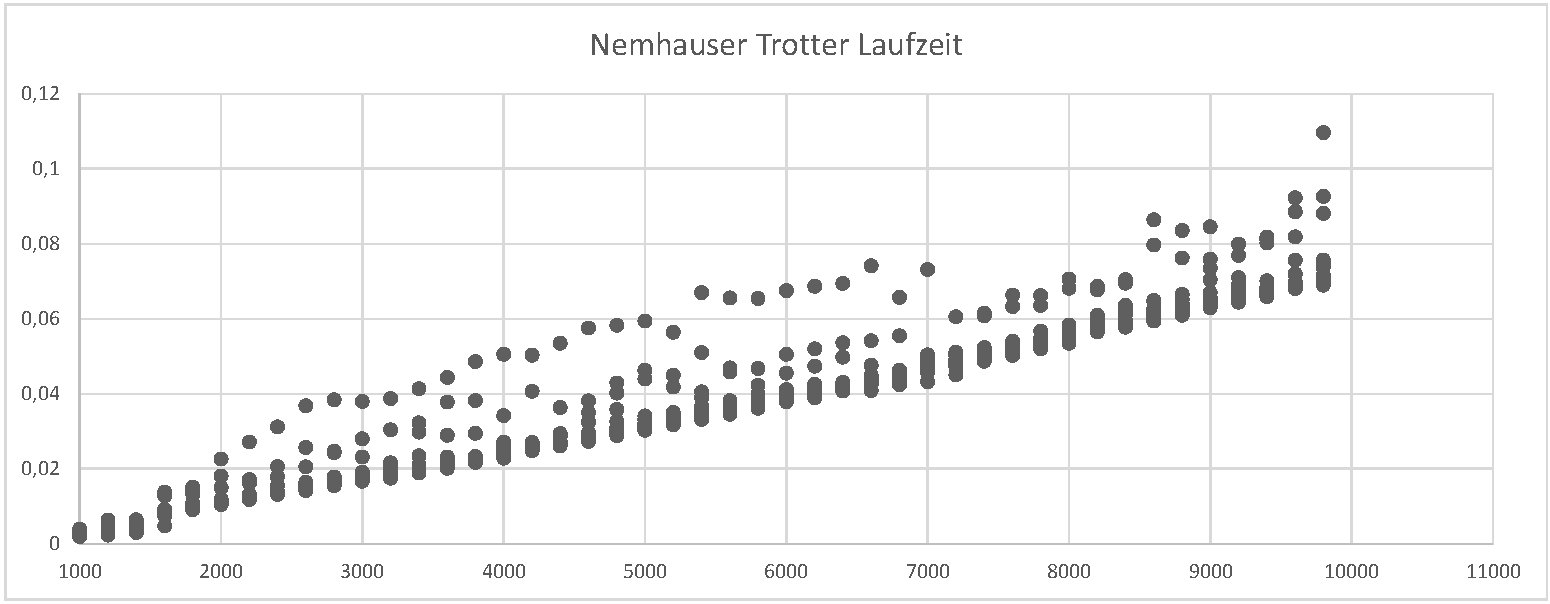
\includegraphics[width=0.7\textwidth]{trottTimeCrop.pdf}}
	\caption{Laufzeit der Nemhauser-Trotter-Regel am Testset\label{fig:trottTime}}
\centering
\end{figure}Wie in Abbildung \ref{fig:trottTime} zu sehen ist, verhält sich die Laufzeit des implementierten Algorithmus' entsprechend der Abschätzung linear zur Eingabe. Jeder Punkt repräsentiert einen Graphen, für den auf der X-Achse die entsprechende Kantenanzahl und auf der Y-Achse die Zeit, wielange ein Durchlauf der Nemhauser-Trotter-Regel im Schnitt für diesen Graphen gebraucht hat in Sekunden an. Selbiges gilt für die Abblidung \ref{fig:crownTime}, allerdings für die Kronenregel.
%% ==============================
\section{Kronenregel}
%% ==============================
\label{ch:Grundlagen:sec:Kronenregel}
Ziel der Kronenregel ist, im Problemgraphen eine Krone zu finden, welche sich folgendermaßen definiert:\\
\textit{Für einen Graphen} $G=(V,E)$ \textit{besteht eine Krone aus} $H \subseteq V\ und\ I \subseteq V\ mit\ H \cap I = \emptyset,\ sodass$ 
\begin{enumerate}
\item $H = N(I),$ 
\item $\textit{I ist ein Indipendent Set, was bedeutet: }\forall v, w \in I\ gilt\ (vw) \notin E\ und$
\item \textit{die Kanten zwischen H und I enthalten ein Matching in dem alle Knoten aus H enthalten sind.}
\end{enumerate}
Ist eine solche Krone gefunden, kann davon die Menge $H$ in eine Knotenüberdeckung für $G$ hinzugefügt werden, um den Graphen um $H$ und $I$ zu reduzieren. Dies ist für das Knotenüberdeckungsproblem sinnvoll, da $I$ ein Independent Set ist und damit keine Kanten untereinander hat. Werden also nur die Nachbarknoten, beziehungsweise $H$ in die Überdeckung aufgenommen, kann man sicher sein, dass keine Kanten vernachlässigt werden. Für die Untersuchung wurde der folgende Algortihmus implementiert:
\begin{singlespace}
\begin{algorithm}[caption={Kronenregel.}, label={alg2}]
$G = (V, E), n:= |V|, m:=|E|, d:= maximaler\ Grad\ der\ Knoten\ aus\ G$
//$M_{1}$ = Maximal Matching von $G$
  $M_{1} \leftarrow \emptyset$
  foreach $e \in E$ do
    $M_{1} \leftarrow M_{1} \cup e$
    Entferne $e$ und $N(e)$ aus der weiteren Betrachtung
  od
$O$ $\leftarrow$ nicht gepaarte Knoten in $M_{1}$
$M_{2}$ $\leftarrow$ Maximum Matching von $B = (O, N(O), \{ uv| u \in O \wedge v \in N(O)\}) $
$I$ $\leftarrow$ nicht gepaarte Knoten aus $O$ in $M_{2}$
$I'  \leftarrow \emptyset$
while $I' \neq I$ do
  $I' \leftarrow I$
  $H \leftarrow N(I)$
  $I \leftarrow I \cup \{\forall u \in O|\exists v\in H\ (uv \in M_{2})\}$
od
return $I$
\end{algorithm}
\end{singlespace}
Um das Maxmimal Matching $M_{1}$ zu erstellen werden im schlimmsten Fall $m \cdot d$ Schritte benötigt, da dann $d$ Nachbarkanten deaktiviert werden. Ist $d = 1$, so wird jede Kante aus $E$ betrachtet, beziehungsweise in $M_{1}$ aufgenommen. Gilt $|M_{1}| > 2k$, so kann für den Graphen keine Knotenüberdeckung  $ \leq k$ gefunden werden. Das Finden der in $M_{1}$ nicht gepaarten Knoten aus $V$ kostet $n$ Schritte. $B$ kann in etwas weniger als $\frac{nd}{2}$ erstellt werden, da $n$ bis zu $k$ kleiner ist, allerdings fällt dies für die Worst Case Abschätzung nicht sehr schwer ins Gewicht. Um das Matching in diesem bipartiten Graphen zu finden, werden wie bei der Nemhauser-Trotter-Regel  $\sqrt{n} \cdot m$ Schritte benötigt. Ist das Matching $M_{2} > k$, so kann für den Graphen keine Knotenüberdeckung  $ \leq k$ gefunden werden. Die Zeilen 8 bis 13 kosten maximal $n \cdot d$, da die Knoten aus $O$ und deren Nachbarknoten überprüft werden müssen. Insgesamt ergibt das eine Abschätzung von:
\begin{align}
&\ m \cdot d + n + \frac{nd}{2} + \sqrt{n} \cdot m + n  + n \cdot d \\
=&\ d (m+n) +2 n + \frac{nd}{2} + \sqrt{n} \cdot m \\
\Rightarrow &\ O(\sqrt{n} \cdot m)
\end{align}
Wieder erhält man $O(\sqrt{n} \cdot m)$, wird $d$ als Kontsante betrachtet, der Algorithmus eignet sich also für eine Vorverarbeitung des Graphen in Polynomialzeit. Für das Matching $M_{1}$ wird ein Maximal Matching vermutlich wegen der schnelleren Laufzeit, als das Finden eines Maximum Matchings in einem allgemeinen Graph verwendet. Allerdeings gibt es nach Blum \cite{paper:8} einen Algorithmus, der ein Maxmimum Matching in einem allgemeinen Graphen in $O(\sqrt{n} \cdot m)$ findet, was die Gesamtlaufzeit der Kronenregel zwar um den Faktor 2 verschlechtern, allerdings eventuell das Ergebnis der Reduktion verbessern würde. Abu-Khzam et al. \cite{paper:7} vermutet, dass das Matching $M_{1}$ einen großen Einfluss auf das Ergenbnis der Reduktion hat, geht aber in seinem Artikel nicht weiter darauf ein. Insgesamt kann mit der Kronenregel ein Problemkern mit einer Knotenmenge von bis zu $3k$ erreicht werden.
\begin{figure}[htb]
\centering
  	{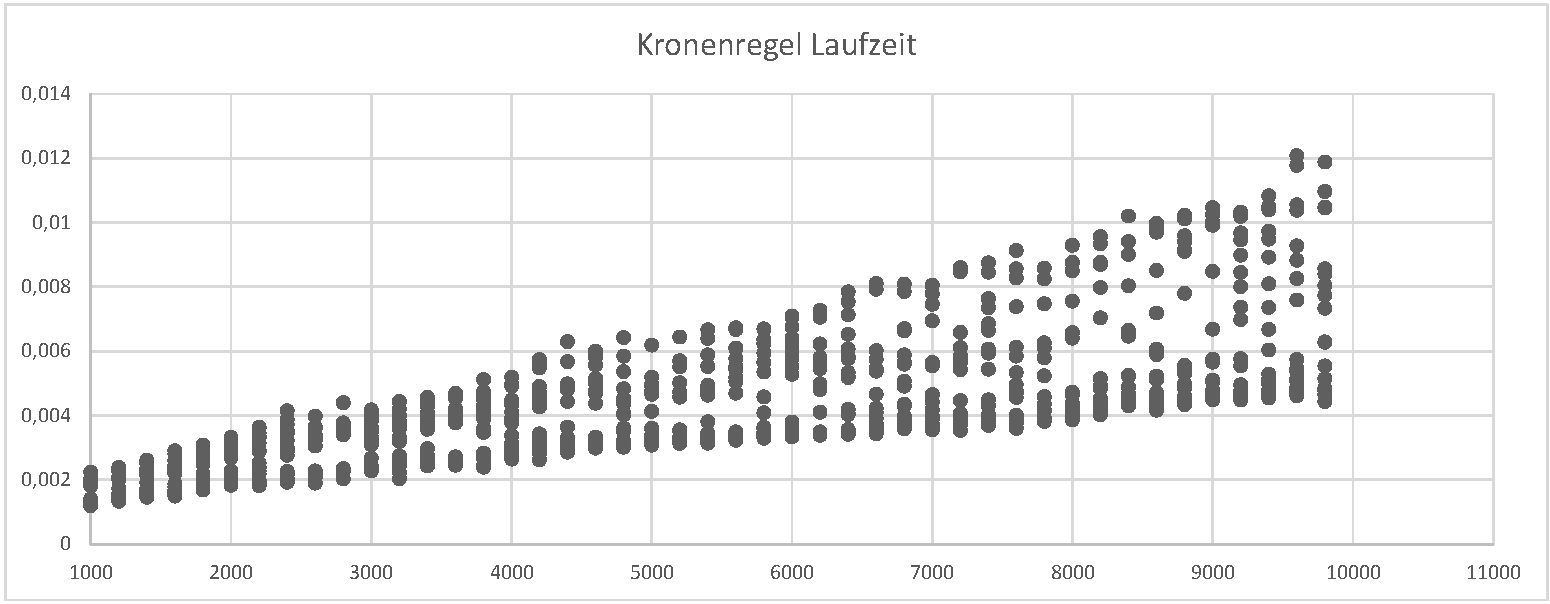
\includegraphics[width=0.7\textwidth]{crownTimeCrop.pdf}}
	\caption{Laufzeit der Kronenregel am Testset\label{fig:crownTime}}
\centering
\end{figure}
Wie in Abbildung \ref{fig:crownTime} zu sehen ist, verhält sich die Laufzeit des implementierten Algorithmus' entsprechend der Abschätzung linear zur Eingabe.
%%% Local Variables: 
%%% mode: latex
%%% TeX-master: "thesis"
%%% End: 
